\documentclass[conference]{IEEEtran}

\usepackage{cite}
\usepackage{amsmath,amssymb,amsfonts}
\usepackage{graphicx}
\usepackage{booktabs}
\usepackage{multirow}
\usepackage{array}
\usepackage{url}
\usepackage{pgfplots}
\usepackage{tikz}
\usepackage[hidelinks]{hyperref}

\pgfplotsset{compat=1.18}
\graphicspath{{figures/}}

\newcommand{\papername}[1]{\textit{#1}}
\newcommand{\scholar}{\papername{scholar\_parser}}
\newcommand{\ocragent}{\papername{ocr\_agent}}
\newcommand{\improvedocr}{\papername{improved\_ocr\_agent}}
\newcommand{\svrocr}{\textsc{SVR-OCR-Full}}
\newcommand{\olmocr}{\papername{olmOCR-2}}
\newcommand{\qwen}{\papername{qwen3-vl-plus}}
\newcommand{\olmbench}{\papername{olmOCR-Bench}}

\begin{document}

\title{\svrocr: Making General-Purpose VLM OCR Competitive for PDF Extraction}

\author{
\IEEEauthorblockN{Siddhant Raje}
\IEEEauthorblockA{\textit{Affiliation to be added for submission}\\
Draft prepared for conference formatting\\
Email to be added for submission}
}

\maketitle

\begin{abstract}
Production document systems often rely on a costly multi-model stack: a general-purpose vision-language model for broader multimodal tasks and a separate specialized OCR model for OCR-heavy pages. This paper focuses on whether a document-aware inference pipeline can make the general-purpose model strong enough to reduce that split. We propose \svrocr, which wraps a general-purpose VLM in typed OCR control, verification, repair, and page-level orchestration instead of relying on direct prompting alone. On \papername{olmOCR-Bench}, \svrocr\ raises the strongest direct Qwen condition from 52.3\% $\pm$ 1.2\% to 72.8\% $\pm$ 1.1\%, a gain of 20.5 points that places it above Mistral OCR (70.9\% $\pm$ 1.0\%) and within 1.5--1.9 points of the stronger specialized OCR baselines we tested, DeepSeek OCR (74.3\% $\pm$ 1.1\%) and \olmocr\ (74.7\% $\pm$ 1.0\%). We study this result in the broader setting of heterogeneous PDF-to-Markdown extraction across born-digital research papers, hybrid reports with screenshots and code, and text-heavy report-style documents. To keep that broader setting visible but secondary, we also construct a manually curated, source-validated benchmark of 120 PDFs and compare three end-to-end systems: \scholar, \ocragent, and a routed hybrid system, \improvedocr. On that internal benchmark, the routed system achieves the strongest overall structure metrics, confirming that OCR backend quality still matters for end-to-end extraction. The main practical implication is that a single general-purpose VLM, when wrapped in the \svrocr\ inference pipeline, can become competitive enough to reduce reliance on a separate specialized OCR backend.
\end{abstract}

\begin{IEEEkeywords}
PDF extraction, document OCR, vision-language models, routing, benchmarking, Markdown conversion
\end{IEEEkeywords}

\section{Introduction}

Modern document pipelines increasingly combine two different kinds of models: a general-purpose vision-language model for broad multimodal tasks and a specialized OCR model for OCR-heavy pages. That split is operationally expensive. It increases serving complexity, endpoint management, routing logic, and the number of models that must be maintained in production. If a single general-purpose VLM could handle both the broader multimodal workload and the OCR branch at competitive quality, the system could be simpler and potentially cheaper to operate.

The obstacle is that direct OCR prompting with a general-purpose VLM still lags behind specialized document OCR systems. Prompt engineering and lightweight cleanup can help, but they do not by themselves solve the hardest OCR cases: dense tiny text, reading order, tables, math-heavy pages, and degraded scans. As a result, a system that wants both broad multimodal competence and strong OCR still tends to deploy multiple models, with the OCR branch treated as a separate specialized subsystem.

This paper is about narrowing that split. We ask whether a general-purpose VLM can be made competitive enough on OCR-heavy pages that a separate OCR-specialized model becomes less necessary. Our answer is \svrocr, an inference-time architecture that wraps the same base general-purpose VLM in typed OCR control, local verification, repair, and page-level orchestration rather than relying on a single direct transcription pass.

The paper still uses heterogeneous PDF extraction as the end-to-end setting, because backend quality only matters if it changes system behavior on real document collections. In that broader setting, different document regimes favor different extraction paths. \scholar\ is stronger on structured scholarly parsing, while \ocragent\ is stronger on some text-heavy and OCR-heavy pages. We therefore retain a routed hybrid system, \improvedocr, as supporting systems context: it demonstrates that OCR backend quality and document regime both matter, but it is not the main claim of the paper.

The central question is therefore not only which routing policy is best, but whether the OCR branch itself can be simplified. For that reason, the paper studies three research questions. \textbf{RQ1}: how does a specialized OCR/document VLM compare with a general-purpose multimodal VLM on OCR-heavy benchmark tasks? \textbf{RQ2}: does category-aware routing improve end-to-end PDF-to-Markdown quality over single-path baselines on heterogeneous documents? \textbf{RQ3}: how far can inference-time improvements make a general-purpose VLM a viable OCR backend inside a routed extraction system?

The central empirical claim of this paper is therefore not merely that routing helps. It is that \svrocr\ improves the strongest direct general-purpose VLM OCR condition by a large margin. On \papername{olmOCR-Bench}, it raises the best direct Qwen result from 52.3\% $\pm$ 1.2\% to 72.8\% $\pm$ 1.1\%, a 20.5-point gain that places it above Mistral OCR and within 1.5--1.9 points of the stronger specialized OCR baselines, DeepSeek OCR and \olmocr. The practical importance of that result is straightforward: if the general-purpose VLM can approach specialized OCR backends closely enough, a single-model deployment becomes more plausible for systems that currently need both.

The paper makes four contributions. First, we propose \svrocr, a document-aware inference pipeline that improves a general-purpose VLM OCR backend through typed OCR control, verification, and repair rather than model retraining. Second, we show on \papername{olmOCR-Bench} that \svrocr\ improves the strongest direct general-purpose VLM OCR baseline by 20.5 benchmark points, outperforms Mistral OCR, and comes within 1.5--1.9 points of DeepSeek OCR and \olmocr. Third, we provide a manually curated 120-document benchmark with source-validated gold annotations for headings, section anchors, figures, and tables so that backend effects can be interpreted in an end-to-end extraction setting. Fourth, we compare three end-to-end systems and show that category-aware routing improves overall extraction quality on heterogeneous PDFs, thereby clarifying where a stronger OCR backend actually matters in a routed document system.

\section{Related Work}

Prior work on PDF extraction and document understanding falls into three groups that are directly relevant here. First, scholarly PDF parsing systems such as GROBID, Science Parse, pdffigures2, and VILA focus on extracting structured content from technical and scientific papers~\cite{grobid,scienceparse,pdffigures2,vila}. These systems established strong baselines for born-digital scholarly parsing, but they are primarily oriented toward scientific documents rather than heterogeneous PDF-to-Markdown extraction across reports, screenshots, and OCR-heavy pages.

Second, recent document OCR and conversion systems increasingly use vision-language models or specialized document pipelines to map PDFs and page images into structured text. Nougat treats scientific PDF extraction as OCR into markup~\cite{nougat}. Docling and Marker are practical open-source conversion toolchains for structured document extraction~\cite{docling,marker}. The \papername{olmOCR} family pushes this direction further with a benchmarked VLM-based PDF text-extraction pipeline for diverse born-digital and scanned PDFs~\cite{olmocr}. More general OCR-oriented VLMs such as GOT-OCR 2.0 argue for unified end-to-end handling of text, math, tables, and charts~\cite{gotocr}. This line of work is the closest background for RQ1 because it treats OCR backend quality as a first-class variable rather than as an implementation detail.

Third, a smaller line of work treats parser choice itself as an adaptive systems problem. AdaParse explicitly assigns parsers to documents and scales resources based on predicted parser suitability~\cite{adaparse}. That idea is close in spirit to our routing question, but our emphasis differs: we study end-to-end PDF-to-Markdown routing across heterogeneous document regimes and then extend that routing story with both an OCR backend study and an inference-time method for improving a general-purpose VLM backend.

\section{Benchmark and Methods}

\subsection{Problem Formulation}

The paper studies PDF-to-Markdown extraction under two coupled objectives. The first objective is end-to-end document fidelity on heterogeneous PDFs: headings should be preserved, section anchors should be assigned to the correct section, and figures and tables should remain attached to the right content structure. The second objective is backend simplification: if a general-purpose VLM can become competitive enough on OCR-heavy pages, the system no longer needs to assume that a separate specialized OCR model is mandatory for mixed multimodal document workloads.

These objectives interact. A routed document system can only be as strong as the backends available to it, and an OCR backend can only be judged fairly if it is evaluated on the kinds of structural OCR cases that actually break downstream extraction quality. For that reason, the paper separates the evaluation into two complementary views. The internal benchmark studies end-to-end document fidelity across heterogeneous full PDFs. The external benchmark studies OCR backend quality directly on OCR-focused page-level tasks. The research contribution is the connection between those views: routing explains where different backends should be used, while \svrocr\ asks how far a general-purpose VLM can be improved before the backend split itself becomes less necessary.

The systems implication is important but should be stated carefully. We do not claim to have measured deployment cost in dollars, GPU-hours, or service-level latency for every model combination. The claim is narrower: if a single general-purpose VLM can approach the specialized OCR backend closely enough, then a single-model deployment becomes more plausible for systems that currently maintain one model for general multimodal work and a separate one for OCR-heavy extraction. The rest of the paper evaluates whether the accuracy evidence is strong enough to support that claim.

\begin{figure*}[t]
\centering
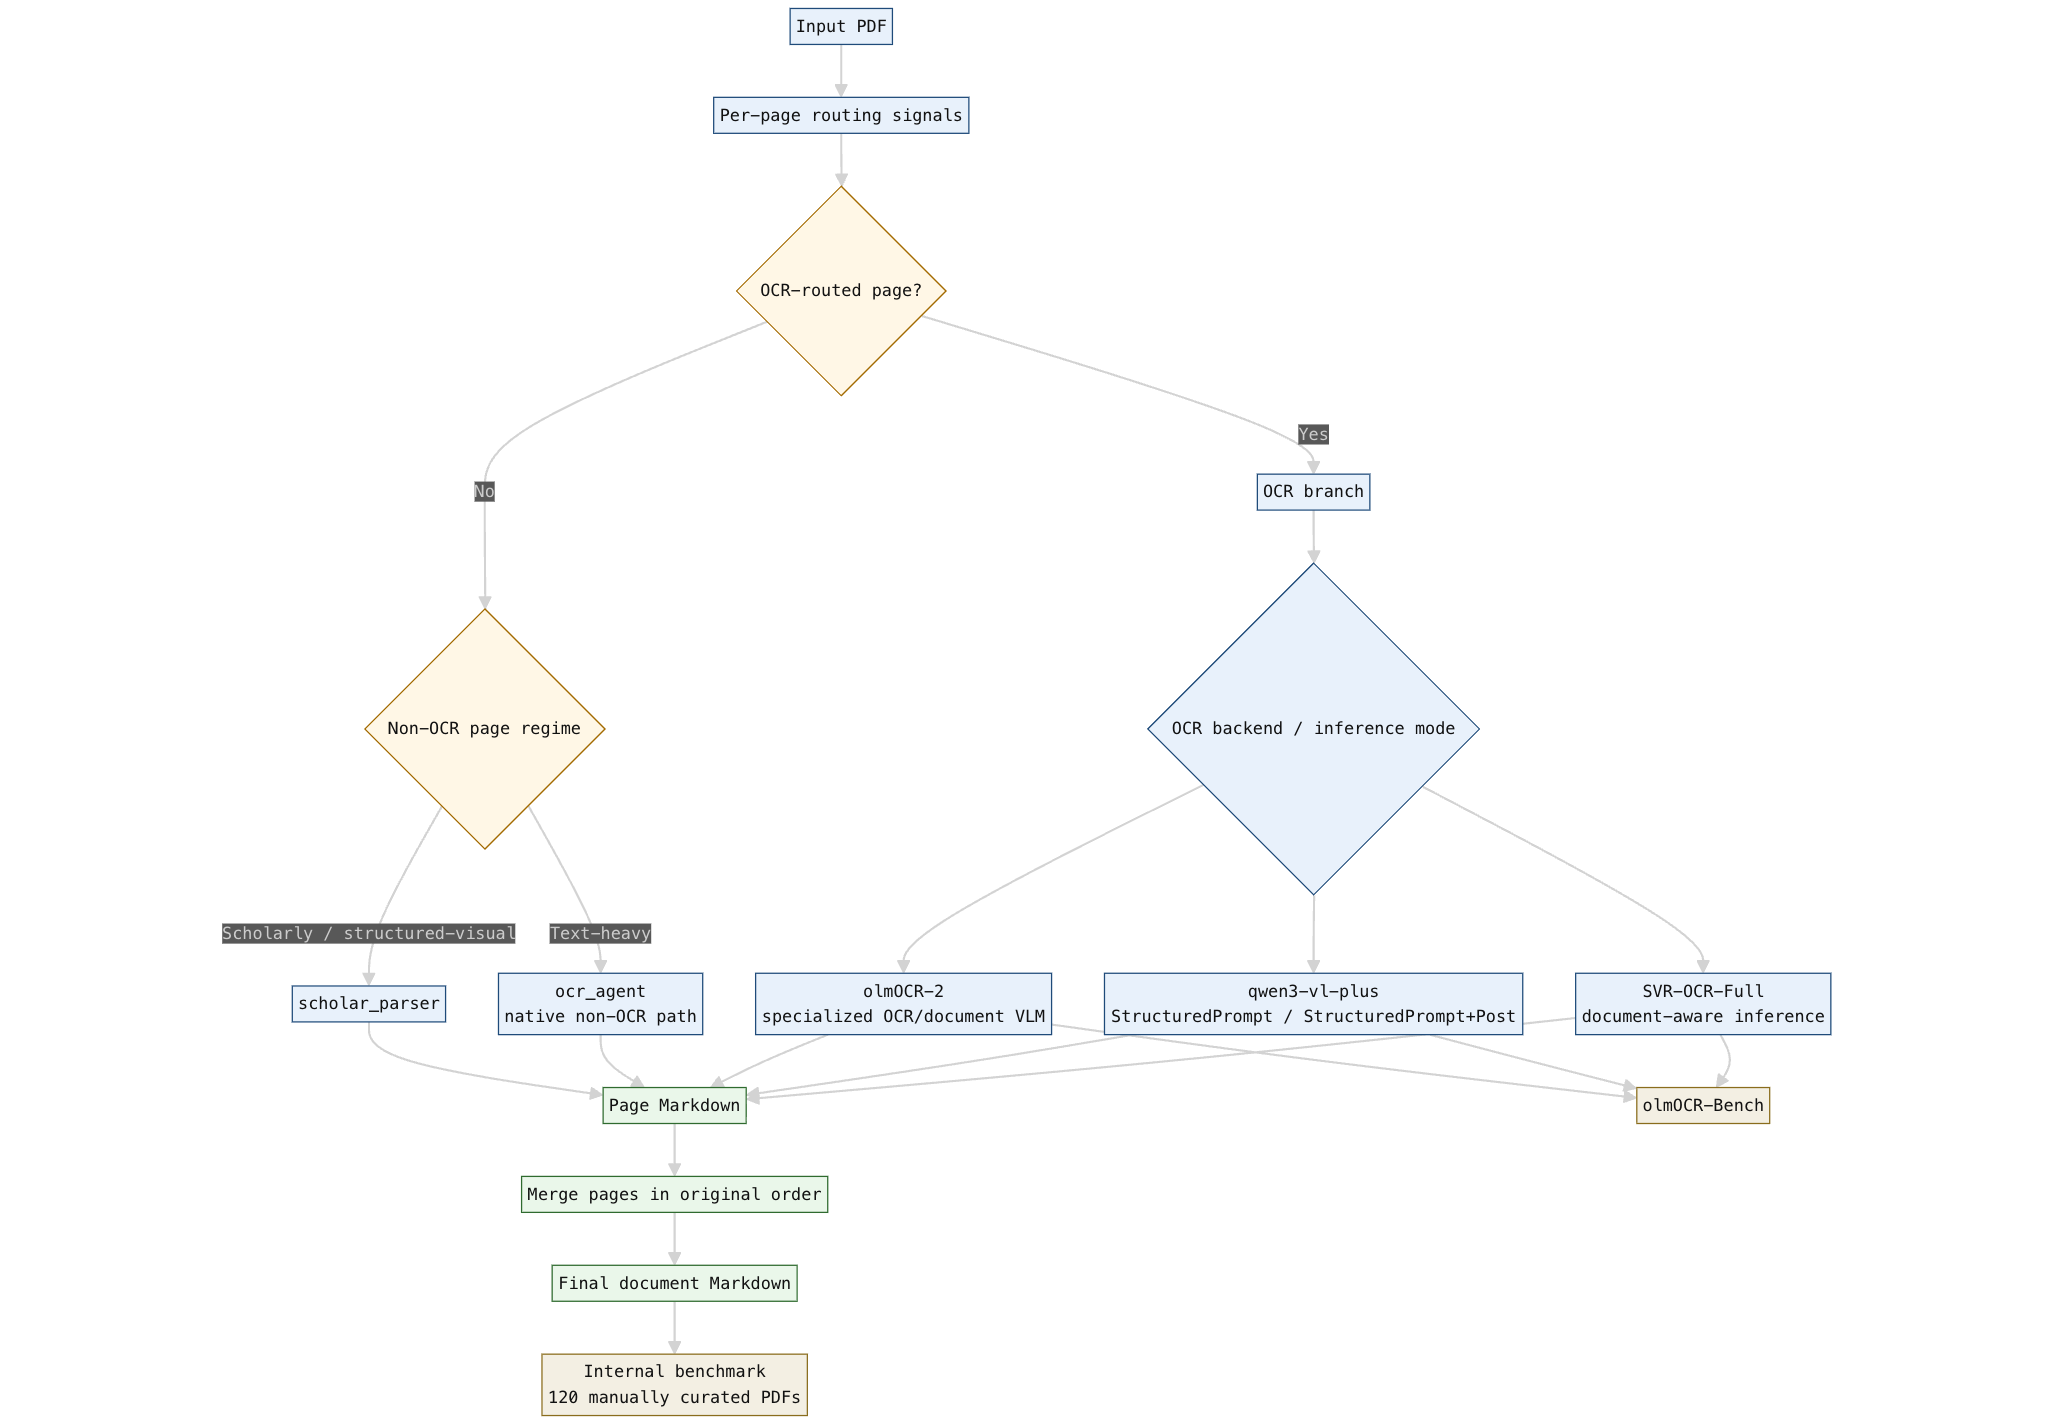
\includegraphics[width=0.98\textwidth]{architecture.png}
\caption{Routed PDF extraction architecture used in the paper. OCR-routed pages remain on the OCR branch, while non-OCR pages are dispatched by document regime. The paper evaluates both end-to-end routing quality and OCR backend quality.}
\label{fig:routed-architecture}
\end{figure*}

\subsection{Internal Benchmark Dataset and Metrics}

Our internal benchmark contains 120 manually curated PDFs divided evenly across three document families: 40 \papername{ResearchPapers}, 40 \papername{Hybrid}, and 40 \papername{TextHeavy}. The benchmark exists to answer a narrower question than \papername{olmOCR-Bench}: if backend quality changes, does it matter in end-to-end PDF-to-Markdown extraction on heterogeneous full documents?

Each document is paired with a gold annotation file created through manual curation against the source PDF. The gold schema includes validated heading lists, section anchor snippets, figure annotations, and table annotations. We therefore evaluate document fidelity rather than raw string similarity. The main internal metrics are heading F1, anchor assignment accuracy, figure recall, and table recall. Anchor assignment accuracy is especially important because it measures whether extracted text appears under the correct section rather than merely appearing somewhere in the output.

\subsection{End-to-End Systems and Routing}

We compare three end-to-end systems, but only as supporting systems context for the \svrocr\ claim. \scholar\ is the project's native structured extraction pipeline and is particularly strong on scholarly parsing, figure extraction, table extraction, and Markdown export quality. \ocragent\ is a hybrid extractor with a VLM-backed OCR path and is stronger on some text-heavy and OCR-heavy cases. \improvedocr\ preserves the original OCR page path but routes non-OCR scholarly or structured-visual pages through \scholar\ while preserving native \ocragent\ handling for non-OCR text-heavy pages. Page outputs are then merged in original page order to produce one final document Markdown file.

\subsubsection{Architecture of Routed PDF Extraction}

Figure~\ref{fig:routed-architecture} shows the routed PDF extraction architecture used in the paper. The key design choice is that OCR-routed pages remain on the OCR branch, while non-OCR pages are dispatched by document regime. Scholarly or structured-visual non-OCR pages go to \scholar, and text-heavy non-OCR pages remain on the native \ocragent\ path. The resulting page outputs are then merged in original document order.

This design matters for two reasons. First, it avoids changing the OCR path itself, which keeps OCR behavior comparable to the original system. Second, it makes the routing logic interpretable: OCR-routed pages stay on OCR, scholarly non-OCR pages use the stronger structured parser, and text-heavy non-OCR pages retain the stronger native report-style handling. The gains of the routed system can therefore be attributed to dispatch choices rather than to a wholesale rewrite of either upstream system.

\subsection{OCR Backends and \svrocr}

At the OCR backend level, the paper studies three conditions. The specialized OCR/document baseline is \olmocr, already integrated into the current OCR flow. The direct general-purpose baseline is \qwen\ under \papername{StructuredPrompt} and \papername{StructuredPrompt+Post}. The strongest inference-time condition is \svrocr, which uses the same general-purpose VLM but wraps it in typed OCR control, provenance tracking, verification, and repair. The intended systems implication is important: instead of pairing a general-purpose VLM with a second specialized OCR model, \svrocr\ asks how far the general-purpose model can be pushed with inference-time structure alone.

\begin{figure*}[t]
\centering
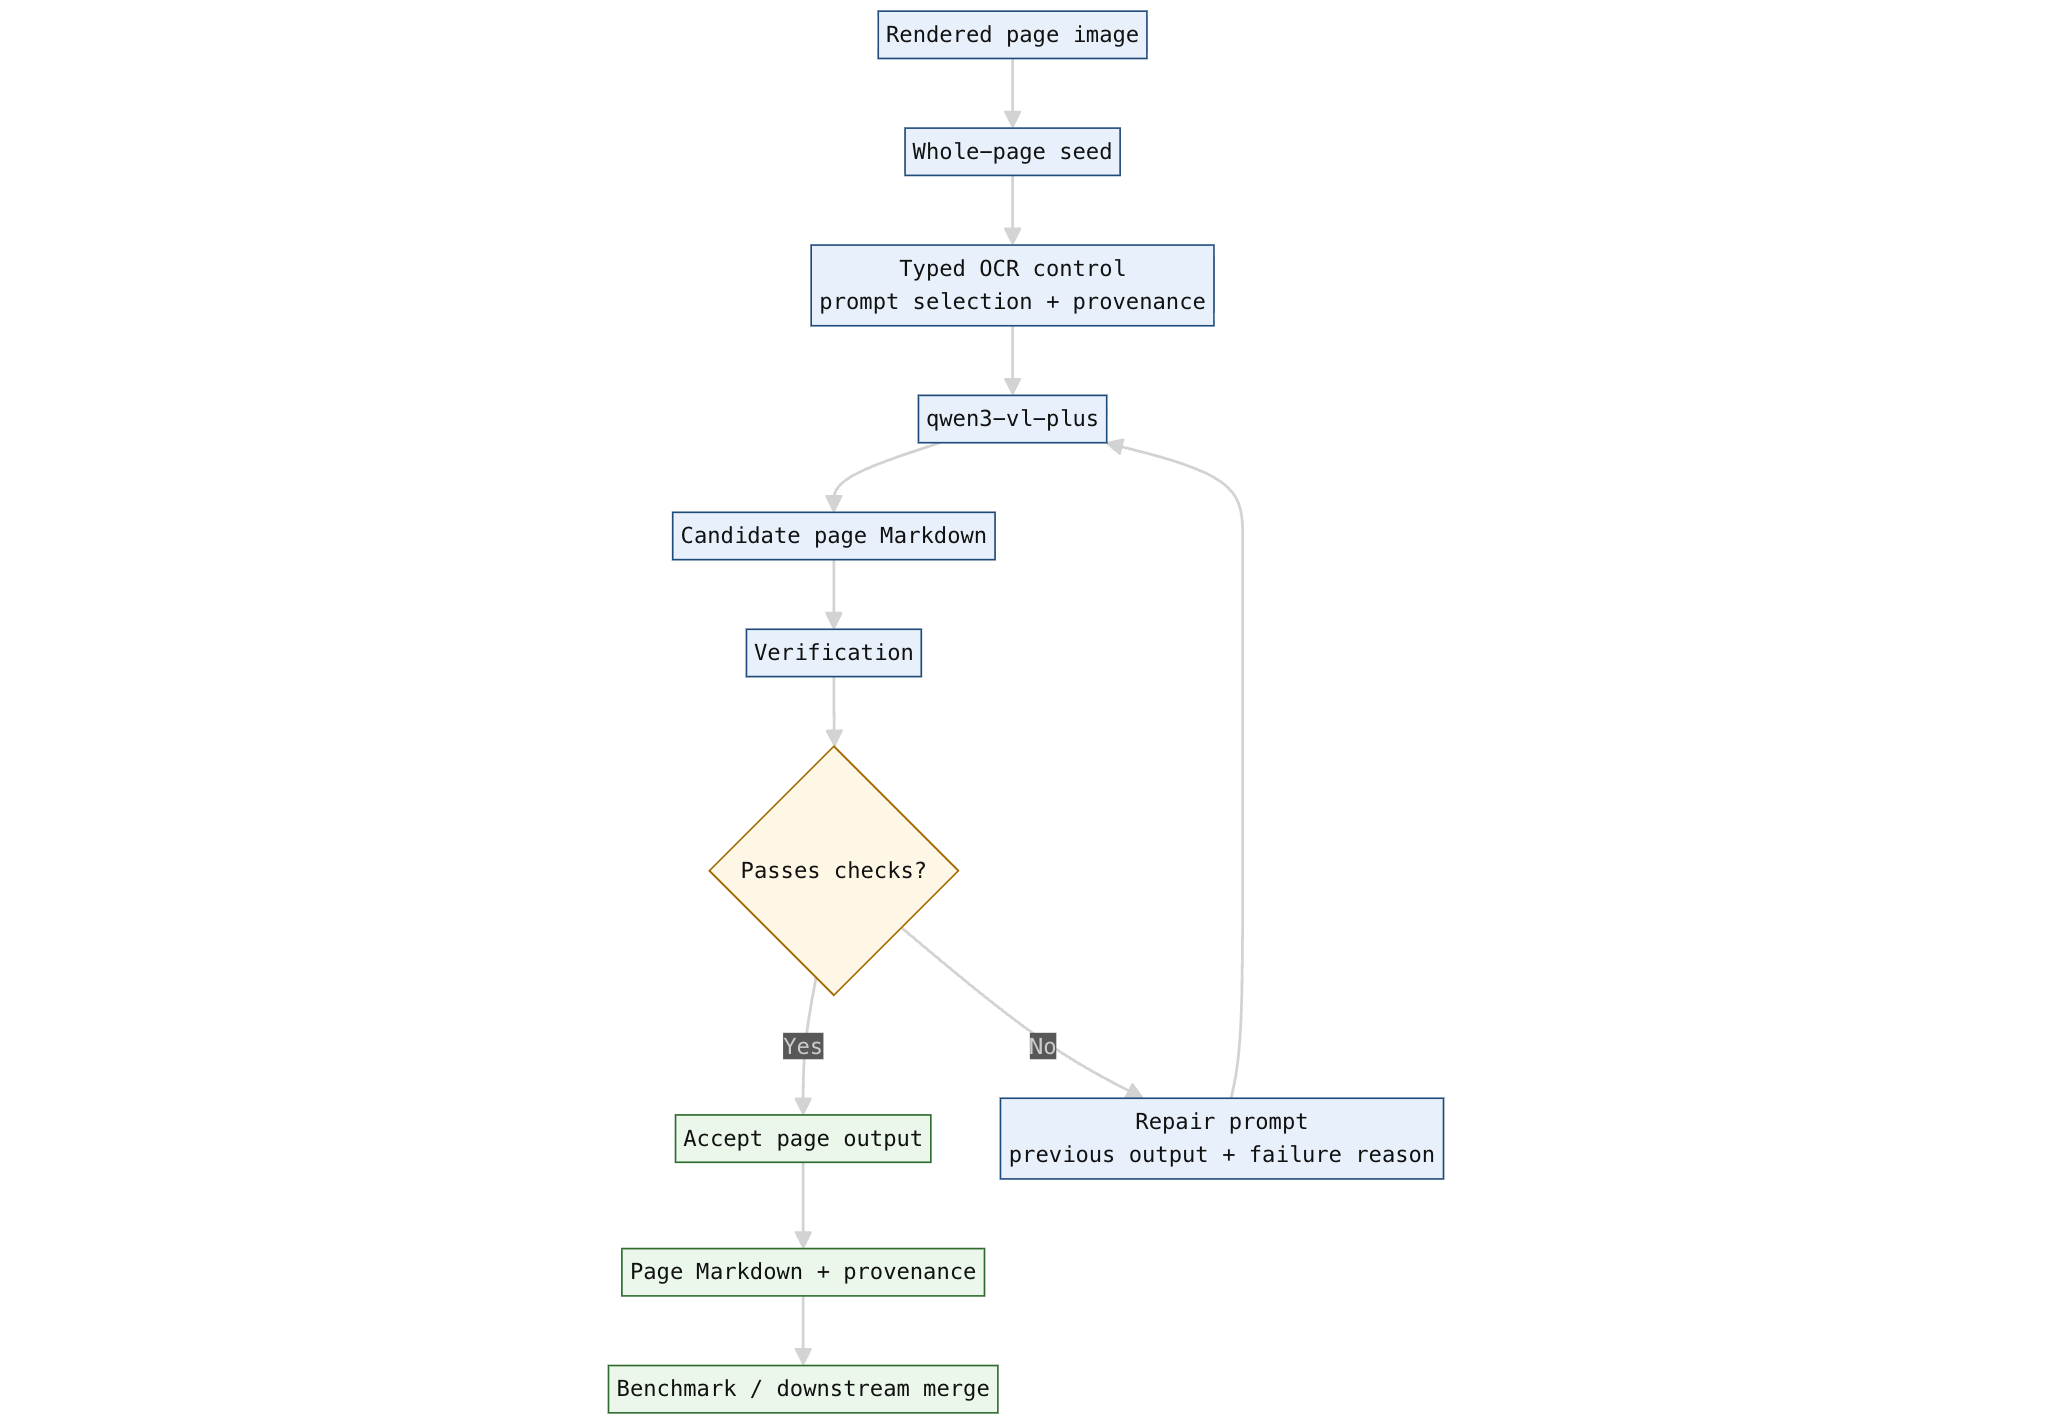
\includegraphics[width=0.92\textwidth]{architecture-svr-ocr.png}
\caption{Current \svrocr\ pipeline. The benchmarked implementation is whole-page seeded and improves the general-purpose VLM through typed OCR control, verification, and repair.}
\label{fig:svr-architecture}
\end{figure*}

\subsubsection{Current \svrocr\ Pipeline}

Figure~\ref{fig:svr-architecture} shows the current \svrocr\ pipeline evaluated in this paper. The page is rendered once, passed through typed OCR control, sent to the same general-purpose VLM used in the direct baseline, and then checked by a verifier that can either accept the output or trigger a repair pass. The final output is therefore not simply the model's first response; it is the verified page-level result of an inference pipeline that explicitly controls and repairs OCR behavior.

\subsubsection{Why Direct Prompting Is Not Enough}

Direct prompting asks a general-purpose VLM to solve OCR as a single pass: read the page, decide the structure, preserve reading order, recover equations, and format the final Markdown correctly, all in one response. The formal benchmark results show the limit of that framing. \papername{StructuredPrompt} and \papername{StructuredPrompt+Post} remain weak on the categories that require explicit document reasoning, including math, tables, multi-column order, and dense tiny text. The problem is therefore not only that the base model needs a better instruction. The problem is that the inference procedure itself is under-structured for document OCR.

\subsubsection{Design Principles of \svrocr}

\svrocr\ is built around three design principles. First, the pipeline should be document-aware: the model should be called under an OCR-specific control policy rather than a generic transcription prompt. Second, the pipeline should be self-checking: low-quality outputs should be detected explicitly rather than accepted as final. Third, the pipeline should be self-repairing: when the first OCR result looks implausible, the system should retry with the previous output and failure reason rather than discarding all context and starting blindly again.

Concretely, the current implementation combines typed OCR control, a page-level verifier, and a repair loop. Typed OCR control selects the OCR contract and tracks provenance for the page. The verifier scores whether the generated output is structurally plausible for the input page. The repair loop re-queries the same model with the previous output plus failure context when the verifier score falls below threshold. This design lets the system spend extra effort only when the first result looks unreliable, instead of rerunning every page indiscriminately.

The benchmarked \svrocr\ implementation is still whole-page seeded. It does not yet represent full block-level layout decomposition. The gain reported in this paper therefore comes from document-aware inference-time control rather than from a new trained OCR model. This distinction is essential to the paper's claim: we are not presenting a newly trained OCR foundation model, but rather a new way of making a general-purpose VLM behave more like a document OCR system at test time.

\section{Experimental Setup}

\subsection{Internal Benchmark Setup}

The internal benchmark evaluates \scholar, \ocragent, and \improvedocr\ on the full 120-document corpus. Each system is run on the full document set, and the resulting Markdown outputs are normalized and compared against manually curated gold annotations for headings, section anchors, figures, and tables. The routed system uses a fixed dispatch policy rather than per-document manual tuning.

For the expanded 120-document rerun reported here, the OCR-backed systems were executed against the same stable managed Qwen endpoint used in the backend study. Earlier internal runs used the native \olmocr\ service, but that endpoint was not available for the full expanded rerun. The internal results should therefore be interpreted as supporting systems evidence under a common managed OCR backend rather than as the main method evaluation.

\subsection{\papername{olmOCR-Bench} Setup}

For backend-only OCR evaluation, we use \papername{olmOCR-Bench}, which contains OCR-focused single-page test cases spanning math, tables, multi-column pages, long tiny text, headers and footers, and historical scans. Candidate generation was run with one repeat per page and benchmarked with the official \papername{olmocr.bench.benchmark} tooling. We report the benchmark's official average score, computed as the average of per-JSONL benchmark-slice scores, together with the associated bootstrap confidence interval. Where helpful, we also report both type-level scores and benchmark-slice breakdowns.

The specialized OCR baseline is \papername{allenai/olmOCR-2-7B-1025-FP8}, served through an OpenAI-compatible \papername{vLLM} endpoint. The general-purpose baseline is \qwen\ evaluated through a stable managed OpenAI-compatible endpoint. This distinction matters operationally because earlier self-hosted experiments were sufficient for pilot runs but not stable enough for the full official benchmark. The formal Qwen-family numbers reported in this paper therefore come from the stable managed-endpoint run.

\subsection{General-Purpose VLM Conditions}

The Qwen-family backend was evaluated under two formal benchmark conditions and one pilot-only condition. The qualitative pilot included \papername{Naive}, \papername{StructuredPrompt}, and \papername{StructuredPrompt+Post}, because that comparison was useful for verifying whether prompt structure mattered at all on full-document examples. The formal \papername{olmOCR-Bench} comparison retained only the two stronger inference-time conditions: \papername{StructuredPrompt} and \papername{StructuredPrompt+Post}.

\papername{StructuredPrompt} uses a document-oriented Markdown transcription prompt aligned with the project OCR pipeline. The prompt requires faithful reading order, heading preservation, conservative math rendering, and structured handling of figures and tables. \papername{StructuredPrompt+Post} uses the same model output but adds deterministic post-processing, including repeated header and footer cleanup, heading normalization, duplicate heading removal, empty-section suppression, and page-order-preserving cleanup. This design keeps the Qwen comparison focused on inference-time improvements rather than retraining.

\subsection{\svrocr\ Evaluation Protocol}

The \svrocr\ evaluation is designed to answer the paper's main question directly: does a document-aware inference pipeline make a general-purpose VLM competitive enough with a specialized OCR backend to reduce the need for a multi-model stack? For that reason, the primary quantitative comparison is not the internal routed-system benchmark. It is the direct-prompting-to-\svrocr\ progression on \papername{olmOCR-Bench}, contextualized by additional specialized OCR baselines including Mistral OCR, DeepSeek OCR, and \olmocr.

This design gives two useful comparisons. The first is the prompt-only progression within the same general-purpose model family, which isolates how much gain comes from adding structure and deterministic cleanup alone. The second is the gap between the strongest direct general-purpose condition and \svrocr, which isolates the value of the inference pipeline itself. The specialized OCR baselines are retained as the ceilings the method is trying to approach. In other words, \papername{olmOCR-Bench} is used here less as a general benchmark leaderboard and more as an instrument for testing whether \svrocr\ meaningfully changes the deployment tradeoff.

\subsection{Reproducibility Notes and Caveats}

Two practical caveats matter for the reported backend study. The final \olmocr\ candidate set still contained 16/1403 empty pages after retry, concentrated in difficult categories such as long tiny text, tables, and headers/footers. The final \svrocr\ candidate set contained 35/1403 empty pages, all in \papername{old\_scans}, due to endpoint-side request-size limits on degraded scan images. Both scores should therefore be interpreted as slightly conservative.

The Qwen-family benchmark results should also be interpreted as the strongest stable managed-endpoint run achieved within the project timeline, not as a claim about every possible self-hosted deployment of the same model family. These caveats affect absolute scores slightly, but they do not change the direction or scale of the comparative result.

\section{Results}

\subsection{Internal Benchmark Results}

The internal benchmark is supporting evidence rather than the center of the paper, so we summarize it briefly. A single-path structured parser is not sufficient across all document regimes, and neither is a single-path OCR-centered system. \scholar\ is strongest on scholarly structure and figure handling, while \ocragent\ is strongest on text-heavy report-like documents. The routed \improvedocr\ produces the best overall balance across the corpus, although the expanded hybrid regime remains unresolved.

\begin{table}[t]
\caption{Overall internal benchmark results on the expanded 120-document corpus.}
\label{tab:internal-overall}
\centering
\footnotesize
\setlength{\tabcolsep}{3pt}
\resizebox{\columnwidth}{!}{%
\begin{tabular}{lcccc}
\toprule
System & Heading F1 & Anchor Acc. & Fig. Rec. & Table Rec. \\
\midrule
\scholar & 0.416 & 0.309 & 1.000 & 0.957 \\
\ocragent & 0.422 & 0.450 & 0.573 & 1.000 \\
\improvedocr & 0.509 & 0.523 & 0.980 & 0.952 \\
\bottomrule
\end{tabular}
}
\end{table}

\begin{figure}[t]
\centering
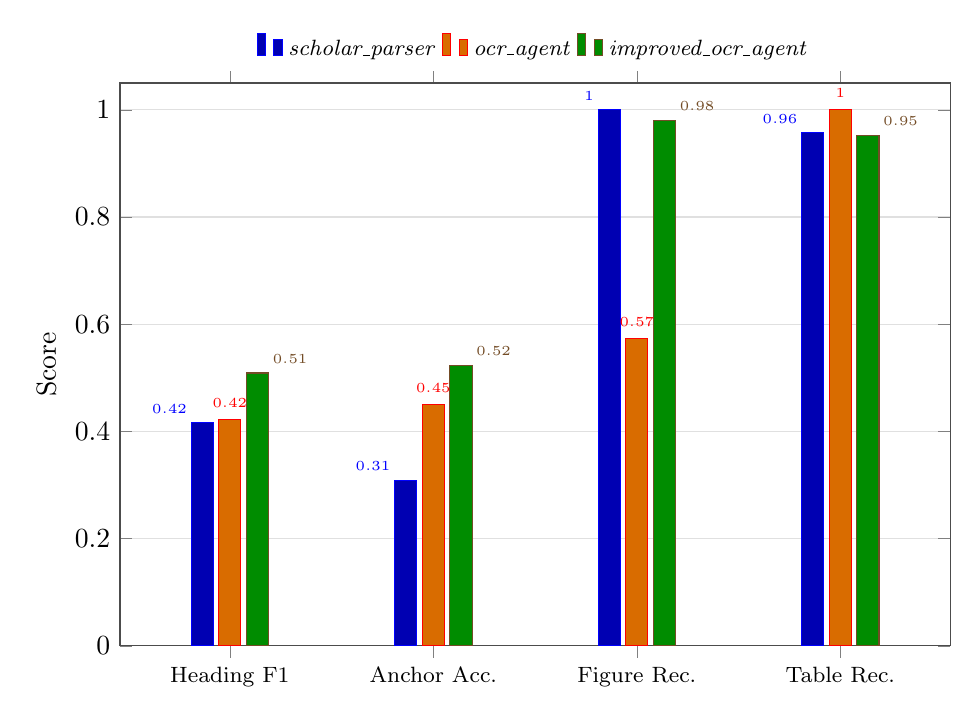
\begin{tikzpicture}
\begin{axis}[
    width=\columnwidth,
    height=0.72\columnwidth,
    ybar,
    bar width=8pt,
    ymin=0,
    ymax=1.05,
    ylabel={Score},
    symbolic x coords={Heading F1,Anchor Acc.,Figure Rec.,Table Rec.},
    xtick=data,
    x tick label style={font=\footnotesize, align=center},
    ytick={0,0.2,0.4,0.6,0.8,1.0},
    legend style={font=\footnotesize, draw=none, at={(0.5,1.02)}, anchor=south, legend columns=3},
    nodes near coords,
    nodes near coords style={
        font=\tiny,
        /pgf/number format/fixed,
        /pgf/number format/precision=2
    },
    enlarge x limits=0.18,
    axis line style={black!70},
    ymajorgrids=true,
    grid style={draw=black!12}
]
\addplot+[
    fill=blue!70!black,
    every node near coord/.append style={anchor=south east, xshift=-2pt}
] coordinates {
    (Heading F1,0.416)
    (Anchor Acc.,0.309)
    (Figure Rec.,1.000)
    (Table Rec.,0.957)
};
\addplot+[
    fill=orange!85!black,
    every node near coord/.append style={anchor=south, yshift=1pt}
] coordinates {
    (Heading F1,0.422)
    (Anchor Acc.,0.450)
    (Figure Rec.,0.573)
    (Table Rec.,1.000)
};
\addplot+[
    fill=green!55!black,
    every node near coord/.append style={anchor=south west, xshift=2pt}
] coordinates {
    (Heading F1,0.509)
    (Anchor Acc.,0.523)
    (Figure Rec.,0.980)
    (Table Rec.,0.952)
};
\legend{\scholar,\ocragent,\improvedocr}
\end{axis}
\end{tikzpicture}

\caption{Overall internal benchmark comparison. The routed system is strongest on the main structure-sensitive metrics while preserving high figure and table recall.}
\label{fig:internal-overall}
\end{figure}

Overall, \scholar\ reaches heading F1 0.416 and anchor assignment accuracy 0.309, with perfect figure recall. \ocragent\ reaches heading F1 0.422 and anchor assignment accuracy 0.450, but with much weaker figure recall. \improvedocr\ improves the overall structure metrics to heading F1 0.509 and anchor assignment accuracy 0.523 while maintaining figure recall 0.980 and table recall 0.952. The takeaway is straightforward: routing helps, and it helps precisely because the OCR branch and the structured parsing branch are not interchangeable.

\begin{table*}[t]
\caption{Per-family internal benchmark results. Heading F1 and anchor assignment accuracy are shown for each document family.}
\label{tab:internal-family}
\centering
\begin{tabular}{lcccccc}
\toprule
& \multicolumn{2}{c}{ResearchPapers} & \multicolumn{2}{c}{Hybrid} & \multicolumn{2}{c}{TextHeavy} \\
\cmidrule(lr){2-3}\cmidrule(lr){4-5}\cmidrule(lr){6-7}
System & Heading F1 & Anchor Acc. & Heading F1 & Anchor Acc. & Heading F1 & Anchor Acc. \\
\midrule
\scholar & 0.684 & 0.572 & 0.156 & 0.127 & 0.407 & 0.229 \\
\ocragent & 0.371 & 0.342 & 0.147 & 0.152 & 0.748 & 0.856 \\
\improvedocr & 0.629 & 0.560 & 0.150 & 0.152 & 0.748 & 0.856 \\
\bottomrule
\end{tabular}
\end{table*}

\begin{figure}[t]
\centering
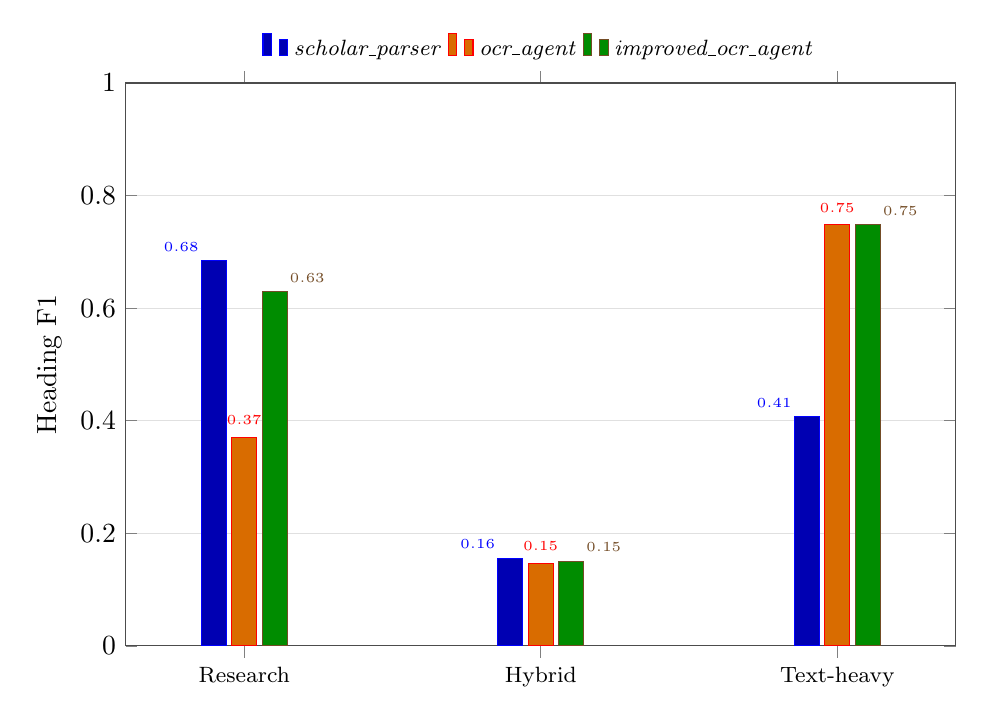
\begin{tikzpicture}
\begin{axis}[
    width=\columnwidth,
    height=0.72\columnwidth,
    ybar,
    bar width=9pt,
    ymin=0,
    ymax=1.0,
    ylabel={Heading F1},
    symbolic x coords={Research,Hybrid,Text-heavy},
    xtick=data,
    x tick label style={font=\footnotesize},
    ytick={0,0.2,0.4,0.6,0.8,1.0},
    legend style={font=\footnotesize, draw=none, at={(0.5,1.02)}, anchor=south, legend columns=3},
    nodes near coords,
    nodes near coords style={
        font=\tiny,
        /pgf/number format/fixed,
        /pgf/number format/precision=2
    },
    enlarge x limits=0.20,
    axis line style={black!70},
    ymajorgrids=true,
    grid style={draw=black!12}
]
\addplot+[
    fill=blue!70!black,
    every node near coord/.append style={anchor=south east, xshift=-2pt}
] coordinates {
    (Research,0.684)
    (Hybrid,0.156)
    (Text-heavy,0.407)
};
\addplot+[
    fill=orange!85!black,
    every node near coord/.append style={anchor=south, yshift=1pt}
] coordinates {
    (Research,0.371)
    (Hybrid,0.147)
    (Text-heavy,0.748)
};
\addplot+[
    fill=green!55!black,
    every node near coord/.append style={anchor=south west, xshift=2pt}
] coordinates {
    (Research,0.629)
    (Hybrid,0.150)
    (Text-heavy,0.748)
};
\legend{\scholar,\ocragent,\improvedocr}
\end{axis}
\end{tikzpicture}

\caption{Heading F1 by document family. The routed system stays close to \scholar\ on research papers and matches \ocragent\ on text-heavy reports, while all systems remain weak on the expanded hybrid set.}
\label{fig:internal-family}
\end{figure}

The per-family breakdown supports the same interpretation. On \papername{ResearchPapers}, \scholar\ remains slightly stronger than the routed system, while on \papername{TextHeavy} documents the routed system exactly matches native \ocragent. On the expanded \papername{Hybrid} set, all systems remain weak. These results justify the claim that backend strengths differ by document regime, but they also show that routing alone does not solve weakly structured hybrid documents.

\subsection{External OCR Backend Study}

\subsubsection{Preliminary Pilot}

Before running the full \papername{olmOCR-Bench} comparison, we ran a controlled three-document pilot on one research paper, one hybrid assignment, and one text-heavy report. In this pilot, \olmocr\ was run on the full PDF directly, while Qwen was run page by page and then merged into one Markdown document per file. Qwen was evaluated under three conditions: \papername{Naive}, \papername{StructuredPrompt}, and \papername{StructuredPrompt+Post}. The pilot is qualitative rather than benchmark-level, but it is informative because it shows where prompt structure helps and where it obviously does not.

On the research paper, naive Qwen was already serviceable, but structured prompting improved heading hierarchy and overall Markdown organization; the post-processed output was the cleanest Qwen variant, although \olmocr\ still preserved tables and structured assets more faithfully. On the hybrid assignment, naive Qwen was not usable as a final output, while structured prompting plus post-processing made the output much more coherent, preserving page structure, screenshots, and some tables; however, \olmocr\ still appeared stronger on mixed visual content. On the text-heavy report, structured prompting alone did not fully solve footer leakage, but the post-processing stage removed those page-footer artifacts and produced a much cleaner final document. Taken together, the pilot established that structured prompting and post-processing were worth carrying into the formal benchmark, but it also suggested that prompt-only Qwen would remain materially weaker than a specialized OCR backend on structural OCR tasks.

\begin{table*}[t]
\caption{Qualitative pilot summary before the formal \papername{olmOCR-Bench} run.}
\label{tab:pilot-summary}
\centering
\begin{tabular}{p{2.6cm}p{3.6cm}p{3.7cm}p{4.1cm}}
\toprule
Document & Best direct Qwen behavior & Relative to \olmocr & Main takeaway \\
\midrule
Research paper & Structured prompting substantially improves section hierarchy and document organization; post-processing yields the cleanest Qwen output. & Competitive on Markdown structure, but weaker on tables and scholarly assets. & General-purpose VLM OCR can handle scholarly text, but specialized OCR still preserves structured assets more faithfully. \\
Hybrid assignment & Naive prompting is not usable; structured prompting and post-processing make the output coherent enough for inspection. & Still weaker on mixed visual fidelity and exactness. & Structured prompting is essential on mixed visual material, but does not eliminate the gap to specialized OCR. \\
Text-heavy report & Post-processing removes repeated footers and produces the best Qwen output. & Competitive and cleaner for Markdown use. & The main early Qwen gain comes from cleaning structure and repeated text, not from solving hard layout or table reasoning. \\
\bottomrule
\end{tabular}
\end{table*}

\subsubsection{\papername{olmOCR-Bench} Results}

The formal \papername{olmOCR-Bench} run sharpens the backend comparison. \olmocr\ remains the strongest overall backend at 74.7\% $\pm$ 1.0\%, and DeepSeek OCR follows closely at 74.3\% $\pm$ 1.1\%. \svrocr\ substantially improves over the strongest direct Qwen baseline and nearly closes the gap to both stronger specialized OCR baselines. The pure prompt-based Qwen conditions reach 50.0\% $\pm$ 1.2\% for \papername{StructuredPrompt} and 52.3\% $\pm$ 1.2\% for \papername{StructuredPrompt+Post}. By contrast, Mistral OCR reaches 70.9\% $\pm$ 1.0\%, \svrocr\ reaches 72.8\% $\pm$ 1.1\%, DeepSeek OCR reaches 74.3\% $\pm$ 1.1\%, and \olmocr\ reaches 74.7\% $\pm$ 1.0\%.

\begin{table*}[t]
\caption{\papername{olmOCR-Bench} type-level results for candidates where per-test-type analysis was collected. Scores are percentages; higher is better.}
\label{tab:olmocr-bench}
\centering
\begin{tabular}{lcccccc}
\toprule
Candidate & Overall & Absent & Math & Order & Present & Table \\
\midrule
\papername{olmocr2} & 74.7 $\pm$ 1.0 & 95.3 & 72.5 & 68.5 & 51.5 & 76.7 \\
\papername{svr\_ocr\_full} & 72.8 $\pm$ 1.1 & 42.3 & 85.4 & 70.7 & 61.2 & 78.2 \\
\papername{qwen\_structured} & 50.0 $\pm$ 1.2 & 67.6 & 45.1 & 38.4 & 16.0 & 44.3 \\
\papername{qwen\_structured\_post} & 52.3 $\pm$ 1.2 & 66.3 & 45.1 & 38.4 & 28.4 & 44.3 \\
\bottomrule
\end{tabular}
\end{table*}

\begin{figure}[t]
\centering
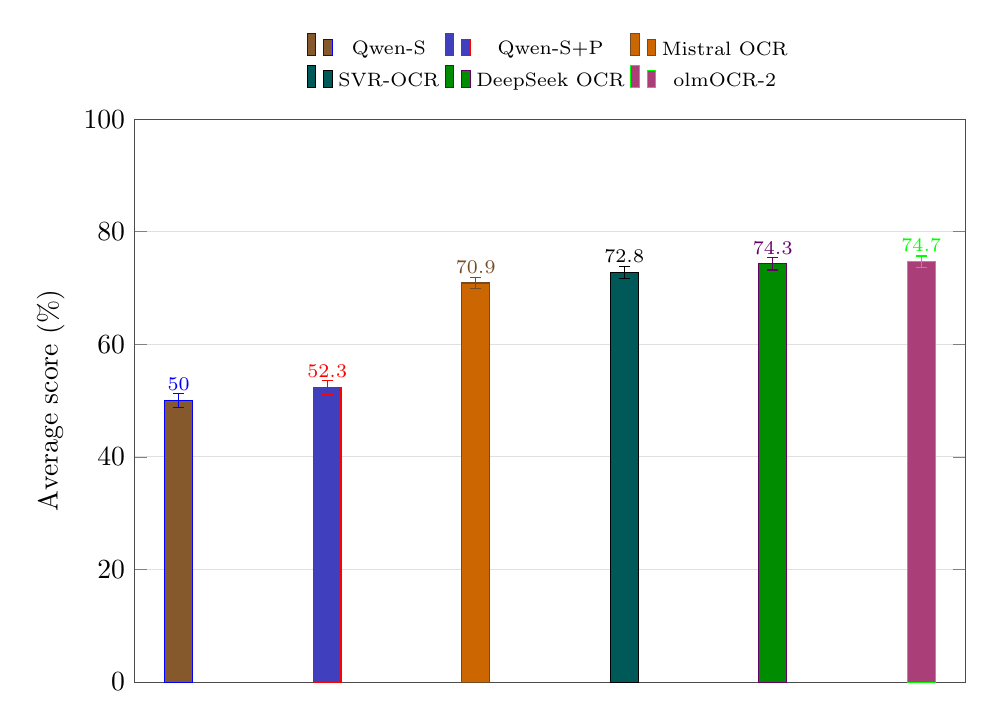
\begin{tikzpicture}
\begin{axis}[
    width=\columnwidth,
    height=0.72\columnwidth,
    ybar,
    bar width=10pt,
    ymin=0,
    ymax=100,
    ylabel={Average score (\%)},
    symbolic x coords={Qwen-S,Qwen-S+P,Mistral OCR,SVR-OCR,DeepSeek OCR,olmOCR-2},
    xtick=\empty,
    ytick={0,20,40,60,80,100},
    nodes near coords,
    nodes near coords style={font=\scriptsize},
    enlarge x limits=0.22,
    axis line style={black!70},
    ymajorgrids=true,
    grid style={draw=black!12},
    legend style={
        font=\scriptsize,
        draw=none,
        at={(0.5,1.03)},
        anchor=south,
        legend columns=3
    }
]
\addplot+[fill=brown!70!black,error bars/.cd,y dir=both,y explicit] coordinates {(Qwen-S,50.0) +- (0,1.2)};
\addplot+[fill=blue!50!gray,error bars/.cd,y dir=both,y explicit] coordinates {(Qwen-S+P,52.3) +- (0,1.2)};
\addplot+[fill=orange!80!black,error bars/.cd,y dir=both,y explicit] coordinates {(Mistral OCR,70.9) +- (0,1.0)};
\addplot+[fill=teal!70!black,error bars/.cd,y dir=both,y explicit] coordinates {(SVR-OCR,72.8) +- (0,1.1)};
\addplot+[fill=green!55!black,error bars/.cd,y dir=both,y explicit] coordinates {(DeepSeek OCR,74.3) +- (0,1.1)};
\addplot+[fill=magenta!65!black,error bars/.cd,y dir=both,y explicit] coordinates {(olmOCR-2,74.7) +- (0,1.0)};
\legend{Qwen-S,Qwen-S+P,Mistral OCR,SVR-OCR,DeepSeek OCR,olmOCR-2}
\end{axis}
\end{tikzpicture}

\caption{Overall \papername{olmOCR-Bench} comparison. \svrocr\ closes most of the gap between direct general-purpose prompting and the stronger specialized OCR baselines we tested.}
\label{fig:backend-overall}
\end{figure}

\begin{figure}[t]
\centering
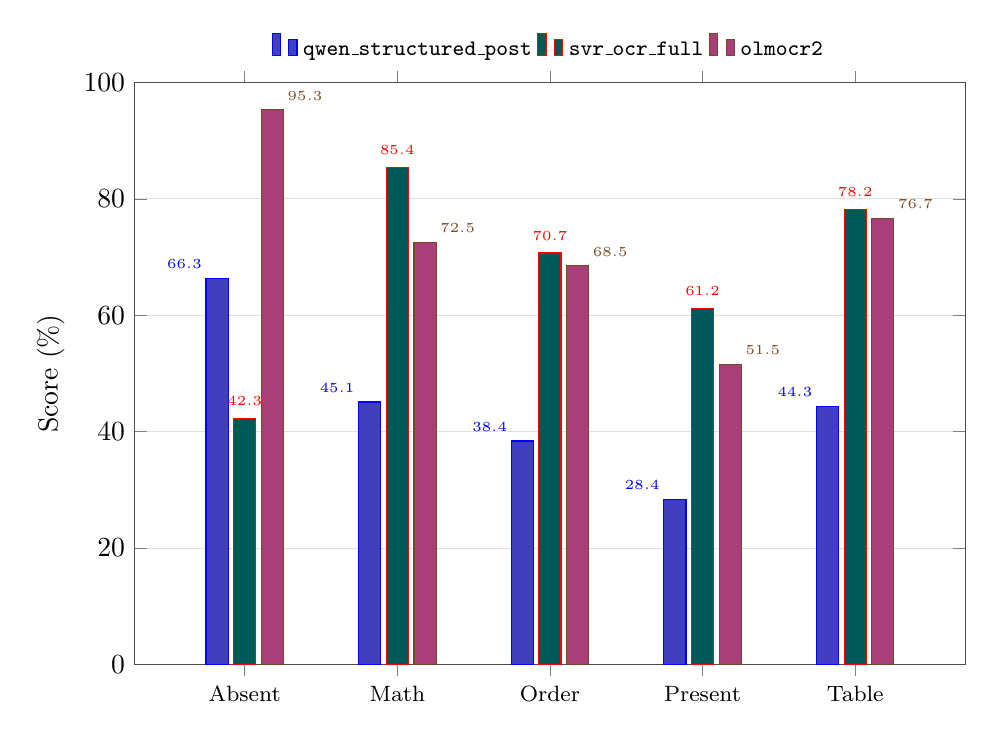
\begin{tikzpicture}
\begin{axis}[
    width=\columnwidth,
    height=0.74\columnwidth,
    ybar,
    bar width=8pt,
    ymin=0,
    ymax=100,
    ylabel={Score (\%)},
    symbolic x coords={Absent,Math,Order,Present,Table},
    xtick=data,
    x tick label style={font=\footnotesize},
    ytick={0,20,40,60,80,100},
    legend style={font=\footnotesize, draw=none, at={(0.5,1.02)}, anchor=south, legend columns=3},
    nodes near coords,
    nodes near coords style={
        font=\tiny,
        /pgf/number format/fixed,
        /pgf/number format/precision=1
    },
    enlarge x limits=0.18,
    axis line style={black!70},
    ymajorgrids=true,
    grid style={draw=black!12}
]
\addplot+[
    fill=blue!50!gray,
    every node near coord/.append style={anchor=south east, xshift=-2pt}
] coordinates {
    (Absent,66.3)
    (Math,45.1)
    (Order,38.4)
    (Present,28.4)
    (Table,44.3)
};
\addplot+[
    fill=teal!70!black,
    every node near coord/.append style={anchor=south, yshift=1pt}
] coordinates {
    (Absent,42.3)
    (Math,85.4)
    (Order,70.7)
    (Present,61.2)
    (Table,78.2)
};
\addplot+[
    fill=magenta!65!black,
    every node near coord/.append style={anchor=south west, xshift=2pt}
] coordinates {
    (Absent,95.3)
    (Math,72.5)
    (Order,68.5)
    (Present,51.5)
    (Table,76.7)
};
\legend{\texttt{qwen\_structured\_post},\texttt{svr\_ocr\_full},\texttt{olmocr2}}
\end{axis}
\end{tikzpicture}

\caption{Type-level \papername{olmOCR-Bench} breakdown for candidates with full test-type analysis. \svrocr\ improves strongly on math, order, present, and table relative to direct prompting.}
\label{fig:backend-category}
\end{figure}

The type-level breakdown shows where the gain comes from. Relative to \papername{qwen\_structured\_post}, \svrocr\ improves on every major benchmark group: math (85.4\% vs. 45.1\%), order (70.7\% vs. 38.4\%), present (61.2\% vs. 28.4\%), and table (78.2\% vs. 44.3\%). It also exceeds \olmocr\ on math, order, present, and table, while remaining much weaker on absent (42.3\% vs. 95.3\%). This view is available only for the candidates for which we collected full per-test-type output analysis.

\begin{figure*}[t]
\centering
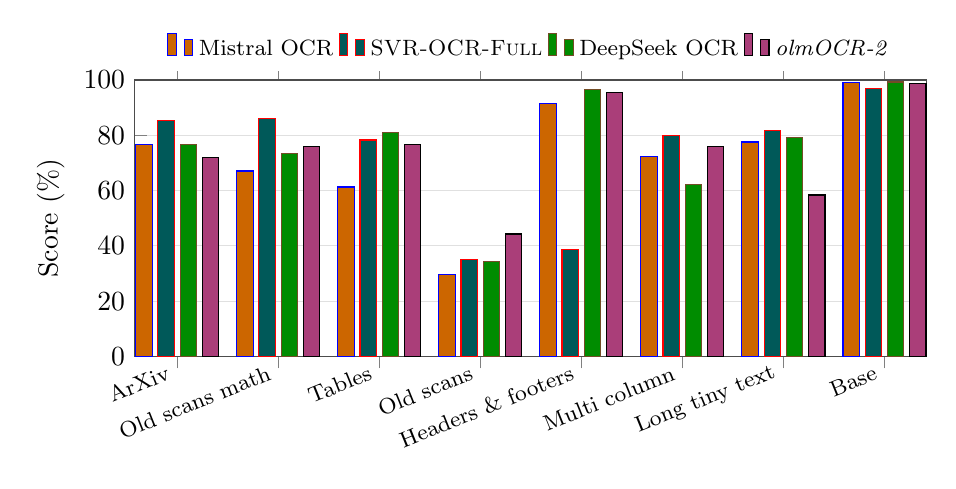
\begin{tikzpicture}
\begin{axis}[
    width=0.96\textwidth,
    height=0.42\textwidth,
    ybar,
    bar width=6pt,
    ymin=0,
    ymax=100,
    ylabel={Score (\%)},
    symbolic x coords={ArXiv,OldScansMath,Tables,OldScans,HeadersFooters,MultiColumn,LongTinyText,Base},
    xtick=data,
    xticklabels={ArXiv,Old scans math,Tables,Old scans,Headers \& footers,Multi column,Long tiny text,Base},
    x tick label style={font=\footnotesize, rotate=22, anchor=east},
    ytick={0,20,40,60,80,100},
    enlarge x limits=0.06,
    axis line style={black!70},
    ymajorgrids=true,
    grid style={draw=black!12},
    legend style={
        font=\footnotesize,
        draw=none,
        at={(0.5,1.03)},
        anchor=south,
        legend columns=4
    }
]
\addplot+[fill=orange!80!black] coordinates {
    (ArXiv,76.7)
    (OldScansMath,67.1)
    (Tables,61.3)
    (OldScans,29.8)
    (HeadersFooters,91.5)
    (MultiColumn,72.3)
    (LongTinyText,77.6)
    (Base,99.2)
};
\addplot+[fill=teal!70!black] coordinates {
    (ArXiv,85.3)
    (OldScansMath,86.0)
    (Tables,78.3)
    (OldScans,35.2)
    (HeadersFooters,38.8)
    (MultiColumn,79.8)
    (LongTinyText,81.7)
    (Base,97.1)
};
\addplot+[fill=green!55!black] coordinates {
    (ArXiv,76.6)
    (OldScansMath,73.5)
    (Tables,81.0)
    (OldScans,34.3)
    (HeadersFooters,96.6)
    (MultiColumn,62.2)
    (LongTinyText,79.1)
    (Base,99.3)
};
\addplot+[fill=magenta!65!black] coordinates {
    (ArXiv,71.9)
    (OldScansMath,76.0)
    (Tables,76.7)
    (OldScans,44.3)
    (HeadersFooters,95.4)
    (MultiColumn,76.1)
    (LongTinyText,58.4)
    (Base,98.8)
};
\legend{Mistral OCR,\textsc{SVR-OCR-Full},DeepSeek OCR,\textit{olmOCR-2}}
\end{axis}
\end{tikzpicture}

\caption{Benchmark-slice comparison across the stronger OCR systems. \svrocr\ is strongest on ArXiv math, old-scans math, multi-column pages, and long tiny text, while DeepSeek OCR is strongest on headers/footers and tables, and \olmocr\ remains strongest on old scans.}
\label{fig:backend-slices}
\end{figure*}

The benchmark-slice breakdown adds another layer to the comparison. \svrocr\ is strongest on \papername{arxiv\_math} (85.3\%), \papername{old\_scans\_math} (86.0\%), \papername{multi\_column} (79.8\%), and \papername{long\_tiny\_text} (81.7\%). DeepSeek OCR is strongest on \papername{headers\_footers} (96.6\%), \papername{table\_tests} (81.0\%), and the baseline group (99.3\%), while \olmocr\ remains strongest on \papername{old\_scans} (44.3\%). Mistral OCR occupies an intermediate position: it is competitive on \papername{arxiv\_math} (76.7\%), \papername{multi\_column} (72.3\%), and \papername{long\_tiny\_text} (77.6\%), but trails the stronger systems on tables and degraded historical scans. This slice-level view matters because it shows that the remaining gap is not uniform: \svrocr\ already matches or exceeds stronger specialized baselines on several mathematically and structurally difficult slices, while still lagging badly on header/footer suppression.

\begin{table*}[t]
\caption{Benchmark-slice pass rates on \papername{olmOCR-Bench}. The official overall score is the average of these per-JSONL slice scores (plus baseline), not the average of the test-type buckets.}
\label{tab:backend-slices}
\centering
\footnotesize
\begin{tabular}{lccccc}
\toprule
Slice & \papername{StructuredPrompt+Post} & \papername{Mistral OCR} & \svrocr & \papername{DeepSeek OCR} & \olmocr \\
\midrule
\papername{arxiv\_math.jsonl} & 41.8 & 76.7 & 85.3 & 76.6 & 71.9 \\
\papername{old\_scans\_math.jsonl} & 66.2 & 67.1 & 86.0 & 73.5 & 76.0 \\
\papername{table\_tests.jsonl} & 44.4 & 61.3 & 78.3 & 81.0 & 76.7 \\
\papername{old\_scans.jsonl} & 31.6 & 29.8 & 35.2 & 34.3 & 44.3 \\
\papername{headers\_footers.jsonl} & 64.7 & 91.5 & 38.8 & 96.6 & 95.4 \\
\papername{multi\_column.jsonl} & 42.6 & 72.3 & 79.8 & 62.2 & 76.1 \\
\papername{long\_tiny\_text.jsonl} & 29.4 & 77.6 & 81.7 & 79.1 & 58.4 \\
\papername{baseline} & 97.8 & 99.2 & 97.1 & 99.3 & 98.8 \\
\bottomrule
\end{tabular}
\end{table*}

These results support two conclusions. First, RQ1 is answered more precisely than in the earlier direct Qwen comparison: the stronger specialized OCR baselines remain ahead overall, but the gap becomes small once the general-purpose model is wrapped in a document-aware inference architecture. Second, RQ3 is no longer limited to the claim that prompting helps somewhat. The completed \svrocr\ run shows that inference-time structure can make a general-purpose VLM genuinely competitive with specialized OCR backends, even though important weaknesses remain in header/footer suppression and degraded old-scan handling.

\subsubsection{From Direct Prompting to \svrocr}

The most important experimental progression in the paper is not simply the final comparison to \olmocr. It is the progression within the general-purpose VLM itself. On \papername{olmOCR-Bench}, the direct prompt-based condition reaches 50.0\% under \papername{StructuredPrompt}. Adding deterministic cleanup raises that to 52.3\% under \papername{StructuredPrompt+Post}. That is useful, but small. By contrast, moving from the strongest direct condition to \svrocr\ raises the score to 72.8\%. In other words, the decisive gain does not come from another prompt variant; it comes from changing the inference architecture around the same base model.

\begin{table}[t]
\caption{Overall \papername{olmOCR-Bench} scores for direct prompting, \svrocr, and additional OCR baselines.}
\label{tab:svr-progression}
\centering
\footnotesize
\begin{tabular}{lc}
\toprule
Condition & Overall score \\
\midrule
\papername{StructuredPrompt} & 50.0 \\
\papername{StructuredPrompt+Post} & 52.3 \\
\papername{Mistral OCR} & 70.9 \\
\svrocr & 72.8 \\
\papername{DeepSeek OCR} & 74.3 \\
\olmocr & 74.7 \\
\bottomrule
\end{tabular}
\end{table}

This is the experimental result that supports the paper's deployment claim. If the score had improved only from 50.0 to 52.3, the conclusion would have been that prompt engineering helps but the multi-model split remains necessary. A jump to 72.8 changes that interpretation. It does not prove that every deployment should immediately discard a specialized OCR model, but it does show that the general-purpose model can be pushed much closer to specialized OCR backends than direct prompting would suggest. In the present runs, \svrocr\ lands above Mistral OCR and within 1.5--1.9 points of DeepSeek OCR and \olmocr.

\subsubsection{\svrocr\ Interpretation}

The benchmark results clarify why the current Qwen-family pipeline remained limited and why \svrocr\ changes the picture. Structured prompting plus post-processing improved difficult text-presence recovery, but it did not materially close the gap on math, reading order, tables, multi-column structure, or long tiny text. \svrocr\ addresses that limitation by adding structured inference-time control around the same general-purpose VLM: typed prompt selection, local verification, repair, and page-level orchestration. The resulting gain is the strongest claim in this paper: \svrocr\ reaches 72.8\% $\pm$ 1.1\%, compared with 52.3\% $\pm$ 1.2\% for \papername{qwen\_structured\_post}, a 20.5-point improvement over the strongest direct general-purpose VLM condition.

\svrocr\ is designed as a document-aware OCR pipeline rather than a single transcription prompt. The full design targets page-layout reasoning, selective refinement of difficult regions, and verifier-guided repair. The benchmarked \svrocr\ implementation reported here represents the first end-to-end version of that idea: it retains whole-page seeding at candidate-generation time, but wraps the VLM call in typed OCR control, provenance tracking, output verification, and repair before final page assembly. This distinction matters because the current results already show a large gain even before full block-level decomposition is introduced.

The key idea is local verification. For each candidate extraction, \svrocr\ evaluates whether the generated output is structurally plausible for the page content and, when needed, triggers a repair pass using the previous output and failure reason. In the broader method design, text blocks can be checked through lightweight rendered-text similarity, table blocks through rendered HTML table structure, and equation blocks through LaTeX rendering. The current benchmarked implementation uses the same principle at the page level and already directly improves the categories where prompt-only Qwen was weakest: math-heavy pages, dense tiny-text recovery, multi-column reading order, and table fidelity.

From a systems perspective, this matters because it changes where the extra computation is spent. A naive retry strategy would simply rerun the whole page blindly. \svrocr\ instead uses verification to decide when the first output is weak enough to justify repair, and it conditions the repair on what went wrong. That makes the method more than a prompt variant and more defensible as a distinct OCR pipeline. It is precisely this shift from one-shot transcription to verifier-guided inference that makes the general-purpose model competitive enough to enter the same conversation as the stronger specialized OCR backends.

\section{Discussion}

Taken together, the results support a single conclusion. On the internal benchmark, category-aware routing remains useful because heterogeneous PDFs benefit from complementary backends rather than a single extraction path, even though the expanded hybrid regime remains difficult. On \papername{olmOCR-Bench}, stronger specialized OCR systems still achieve the highest overall scores, but the gap is now small once a general-purpose VLM is wrapped in \svrocr: the method improves the strongest direct Qwen condition from 52.3\% $\pm$ 1.2\% to 72.8\% $\pm$ 1.1\%, surpasses Mistral OCR, and comes within 1.5--1.9 points of DeepSeek OCR and \olmocr. The broader implication is that prompt cleanup alone is not enough, whereas document-aware inference with explicit control, verification, and repair can make a general-purpose VLM a genuinely competitive OCR backend for mixed document systems.

This matters operationally. A general-purpose VLM that becomes competitive on OCR-heavy pages can reduce dependence on a separate specialized OCR backend, which in turn can simplify deployment for mixed multimodal workloads. We do not claim to have measured the dollar cost of that simplification directly. The claim is narrower and more defensible: the accuracy gap is now small enough that a single-general-purpose-VLM deployment becomes plausible in situations where the multi-model split was previously justified primarily by OCR quality. That is the real paper-level implication of the 20.5-point gain: the comparison is no longer between a weak general-purpose OCR baseline and a strong specialized model, but between a nearly competitive general-purpose pipeline and several specialized OCR backends that still hold a smaller remaining edge.

\section{Implementation Note}

The formal Qwen-family benchmark conditions were implemented through the benchmark runner's project prompt templates rather than through ad hoc manual prompting. The simplest pilot condition corresponds to a naive transcription contract: transcribe the page to Markdown, preserve visible text in reading order, and do not summarize. The stronger benchmark condition, \papername{StructuredPrompt}, follows the project OCR contract more closely. Operationally, the prompt requires the model to return a faithful Markdown transcription in natural reading order while preserving headings, paragraphs, lists, captions, references, and footnotes; removing clearly repetitive headers and footers; converting equations to LaTeX; using HTML for tables; avoiding hallucinated content; and emitting figure placeholders in a fixed Markdown image-reference format when image regions should be preserved.

The \papername{StructuredPrompt+Post} condition uses the same model output but adds a deterministic cleanup pass. The post-processing recipe has seven fixed steps: parse the YAML front matter; strip obvious repeated headers and footers; normalize heading markers and numbering prefixes; remove duplicate headings; remove empty sections unsupported by body text; normalize figure and table placeholder formatting; and preserve page order without merging content across pages. This matters methodologically because the gain attributed to \papername{StructuredPrompt+Post} is not the result of retraining or hand-editing. It is a strictly inference-time improvement applied uniformly across outputs.

\section{Limitations and Error Analysis}

The paper has three important limitations. First, the final \svrocr\ candidate set still contained 35/1403 empty pages, all in \papername{old\_scans}, due to endpoint-side request-size limits on degraded scan images. The reported 72.8\% should therefore be interpreted as slightly conservative. Second, the current benchmarked \svrocr\ implementation is still whole-page seeded. The results already show a large gain from typed OCR control, verification, and repair, but they do not yet represent full block-level layout decomposition. Third, the expanded hybrid regime remains weak across all three end-to-end systems, which indicates that routing alone does not solve weakly structured, visually irregular hybrid documents.

The backend failure profiles are also informative. The direct Qwen post-processed condition fails 3904 tests, \olmocr\ fails 1910, and \svrocr\ fails 1821. The direct general-purpose condition fails broadly on structural OCR categories, especially math, order, table, and present. By contrast, \svrocr\ shifts the remaining burden toward absent, degraded scan behavior, and the tail of the benchmark rather than failing uniformly across all structural categories.

The benchmark slices make that pattern concrete. Qwen-family failures are concentrated in exactly the categories that require document-aware structure recovery: dense tiny text, multi-column reading order, and table fidelity. Representative order failures show the model interleaving distant column fragments rather than preserving local reading sequence. Representative table failures show partial cell recovery without a stable grid. Representative math failures show long expressions or operator-rich lines being dropped or normalized into non-matching forms. By contrast, \olmocr\ still fails on very difficult math-heavy and degraded historical pages, but those failures are more concentrated at the extreme end of the benchmark rather than spread broadly across structural categories.

The internal benchmark shows the same regime dependence at the document level. On scholarly papers such as \papername{p118} and \papername{p119}, the routed system stays close to \scholar, while plain \ocragent\ loses meaningful structure. On \papername{p118}, \scholar\ and \improvedocr\ both remain above 0.92 heading F1, whereas \ocragent\ drops to 0.560 heading F1 and 0.207 anchor assignment accuracy. On \papername{p119}, the routed system nearly preserves the \scholar\ result, while \ocragent\ weakens anchor assignment from 0.889 to 0.556. These examples show that born-digital research PDFs reward strong structured parsing and careful section assignment, not only raw text recovery.

The hybrid and text-heavy examples expose a different limitation. On structured assignments such as \papername{a005}, \papername{a006}, and \papername{a007}, \scholar\ and \improvedocr\ remain strong while plain \ocragent\ loses both headings and anchors. On visually irregular hybrid reports such as \papername{a008} and \papername{a009}, however, all systems score poorly on heading F1, and even the routed system does not recover a stable hierarchy. In those cases, the problem is not only backend choice; the documents themselves are weakly heading-structured and visually dominated by mixed content. On the text-heavy report \papername{t001}, the pattern flips: \scholar\ is weak, while both \ocragent\ and \improvedocr\ achieve strong heading and anchor performance. Taken together, the error analysis reinforces the paper's main claim: the hard cases are not random outliers. They are systematic manifestations of document regime.

\section{Conclusion}

This paper studied PDF-to-Markdown extraction as both a systems problem and a backend problem, but its main contribution is at the backend level. Modern document systems often maintain one model for general multimodal tasks and another for OCR-heavy pages because direct general-purpose VLM OCR is too weak. \svrocr\ changes that picture by replacing direct prompting with a document-aware inference pipeline built around typed OCR control, verification, and repair.

On \papername{olmOCR-Bench}, the strongest specialized backends in our runs are \olmocr\ at 74.7\% $\pm$ 1.0\% and DeepSeek OCR at 74.3\% $\pm$ 1.1\%, while \svrocr\ raises the strongest direct general-purpose VLM condition from 52.3\% $\pm$ 1.2\% to 72.8\% $\pm$ 1.1\%, a gain of 20.5 points that also places it above Mistral OCR at 70.9\% $\pm$ 1.0\%. The internal routed-system benchmark then provides the supporting systems context: backend strengths differ strongly by document regime, and a stronger OCR branch matters because heterogeneous PDFs benefit from routing rather than single-path extraction.

The present evidence therefore suggests a more practical deployment story than the one with which the paper began. A document-aware inference architecture can make a single general-purpose VLM strong enough to cover both broader multimodal tasks and OCR-heavy extraction more plausibly than direct prompting alone, while still leaving room for specialized models in the hardest cases. That is a stronger and more actionable conclusion than merely observing that prompt engineering helps. It says that the gap between general-purpose and specialized document OCR can be narrowed substantially through inference-time design, and that future document systems should treat this as a serious alternative to the default multi-model split.

\bibliographystyle{IEEEtran}
\bibliography{references}

\end{document}
